\frame{\frametitle{Massive stars ($>8M_\odot$) are significant because they produce a large fraction of the heavy elements either during their evolution or in supernovae.}
\begin{figure}[h]
	\centering
		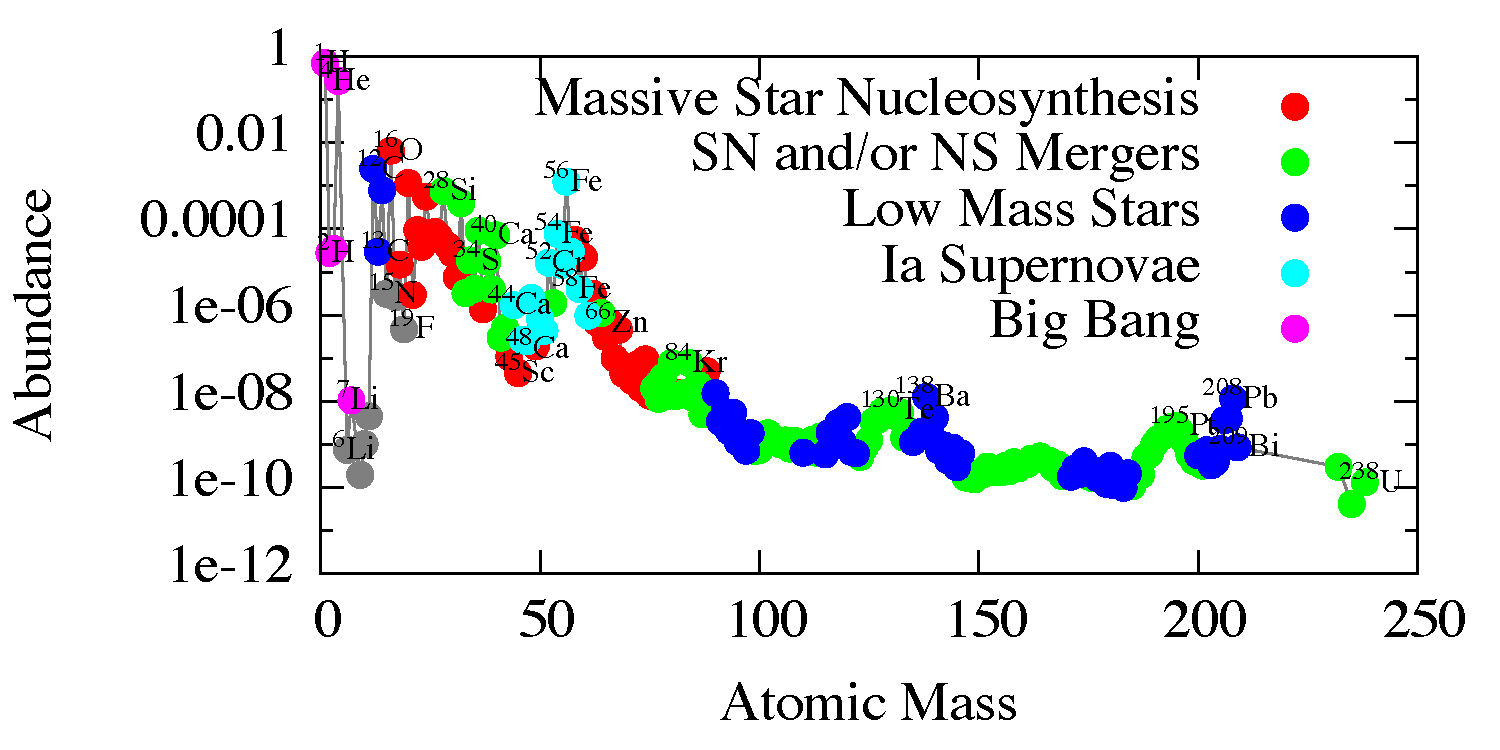
\includegraphics[width=.9\textwidth]{figs/abundances.pdf}\footnote{\citep{Lodders2010,Woosley2002,Burbidge1957}}
	\label{fig:figs_abundances}
\end{figure}
}

\frame{\frametitle{Stellar evolution codes need to run a simulated time spanning from millions to billions of years.}
\begin{figure}
	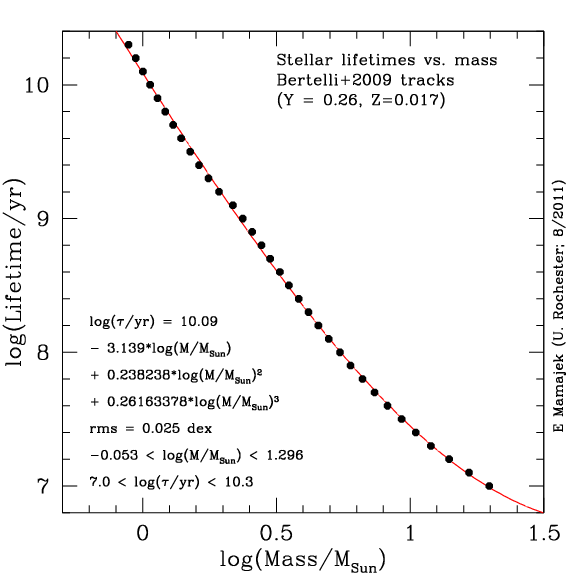
\includegraphics[width=0.4\columnwidth]{stellar_lifetimes.png}
\end{figure}
Since we can only model this in 1D, we need models for 3D processes.
}

\frame{\frametitle{Much effort has been spent to understand normal convection, but minor mixing processes get less attention.}
\begin{figure}
	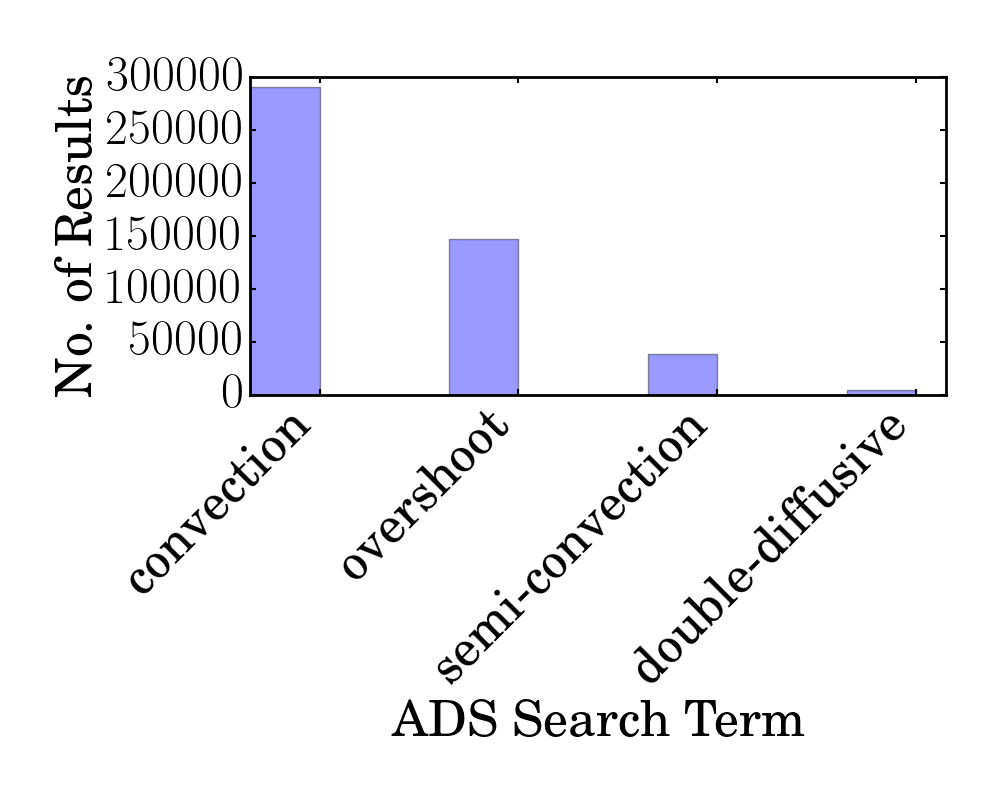
\includegraphics[width=0.8\columnwidth]{ads.png}
\end{figure}
}

\frame{\frametitle{Since the later stages of massive stars are complex, small changes can have major effects.}
\begin{figure}[h]
	\centering
		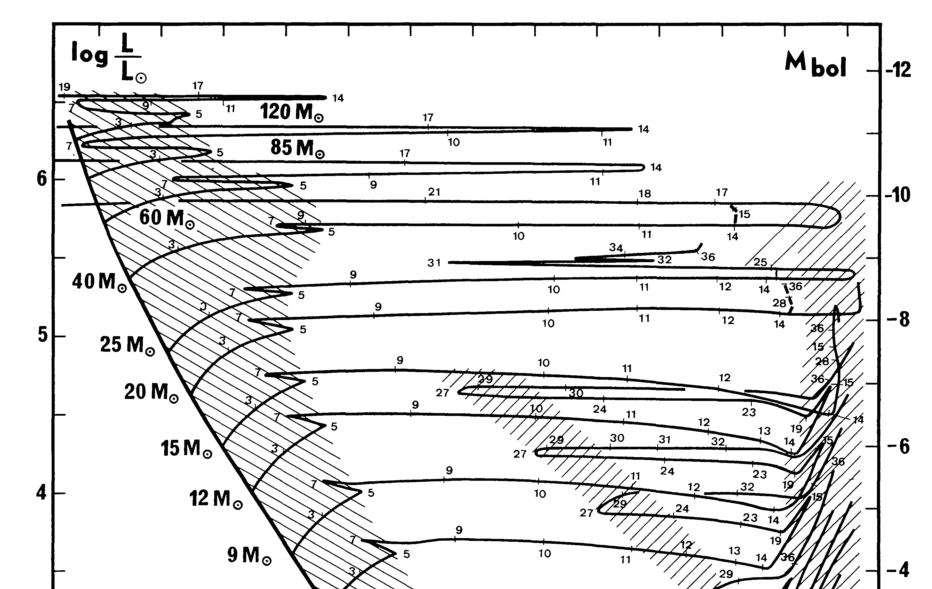
\includegraphics[width=.8\textwidth]{figs/Maeder-HR-head.png}

		\hspace{7pt}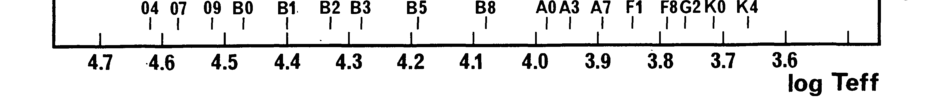
\includegraphics[width=.8\textwidth]{figs/Maeder-HR-foot.png}\footnote{\citep{Maeder1988}}
	\label{fig:figs_himasshr}
\end{figure}
}

\frame{\frametitle{Since these late stages are dynamic, mixing processes (e.g. semi-convection) can drastically effect the final star structure and yields.}
\begin{figure}[h]
	\centering
		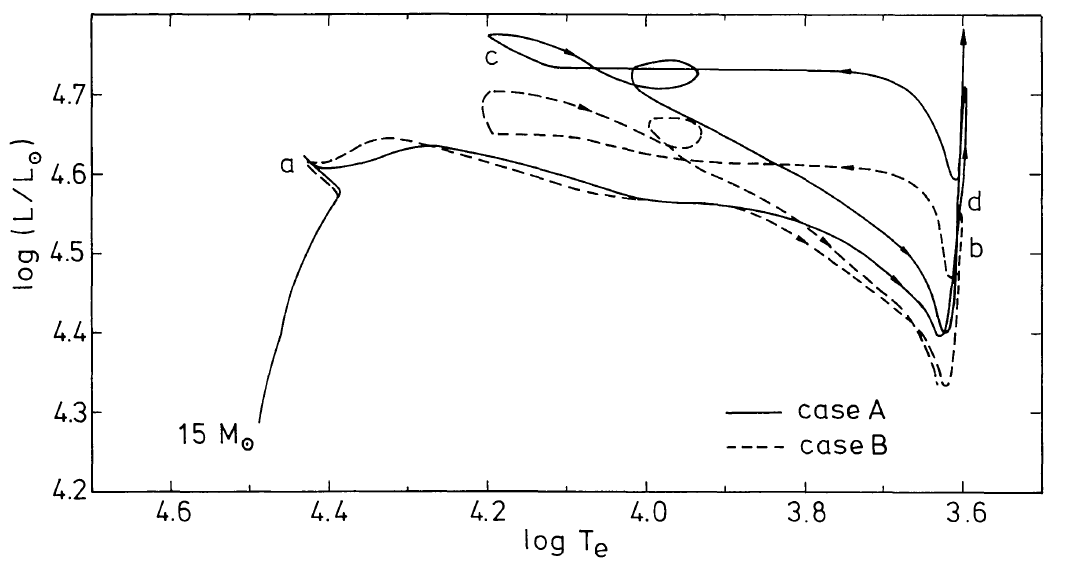
\includegraphics[width=.7\textwidth]{figs/semi_evolution.png}\footnote{\citep{Langer1985}}
		\caption{With semi-convection (solid), without (dashed)}
	\label{fig:figs_semi_evolution}
\end{figure}
}

\frame{\frametitle{These processes, in particular overshooting convection and double-diffusive mixing can substantially affect the results.}
\begin{figure}
	\includegraphics[width=1.0\columnwidth]{he_mass_param.pdf}
\end{figure}
}